\documentclass[conference]{IEEEtran}
\IEEEoverridecommandlockouts
% The preceding line is only needed to identify funding in the first footnote. If that is unneeded, please comment it out.
\usepackage{cite}
\usepackage{amsmath,amssymb,amsfonts}
\usepackage{algorithmic}
\usepackage{graphicx}
\usepackage{textcomp}
\usepackage{xcolor}
\def\BibTeX{{\rm B\kern-.05em{\sc i\kern-.025em b}\kern-.08em
    T\kern-.1667em\lower.7ex\hbox{E}\kern-.125emX}}
\begin{document}

\title{KUKA LBR iiwa --- Adaptive Assembly Analysis}

\author{\IEEEauthorblockN{Arjan Gupta}
\IEEEauthorblockA{\textit{Robotics Engineering} \\
\textit{Worcester Polytechnic Institute}\\
Worcester, MA, USA \\
agupta11@wpi.edu}
}

\maketitle

\begin{abstract}
This paper presents an analysis of the KUKA LBR iiwa robot's
ability to perform rigid-body assembly tasks. The analysis is based on the first YouTube
video presented in the prompt of the final exam. The video shows the robot's ability
to adapt to the environment and perform manufacturing assembly tasks.
\end{abstract}

\begin{IEEEkeywords}
KUKA, LBR iiwa, assembly, analysis
\end{IEEEkeywords}

\section{Introduction}
The KUKA LBR iiwa robot is a 7-axis robot that is capable of performing 
rigid-body assembly tasks, as shown in the YouTube video~\cite{youtube_2014}. As per the data sheet
of the robot, it is capable of performing assembly tasks with a payload of 7--14 kg,
depending on the model.
Its maximum reach is 800--820 mm depending on the model.

\begin{figure}[h!]
\centering
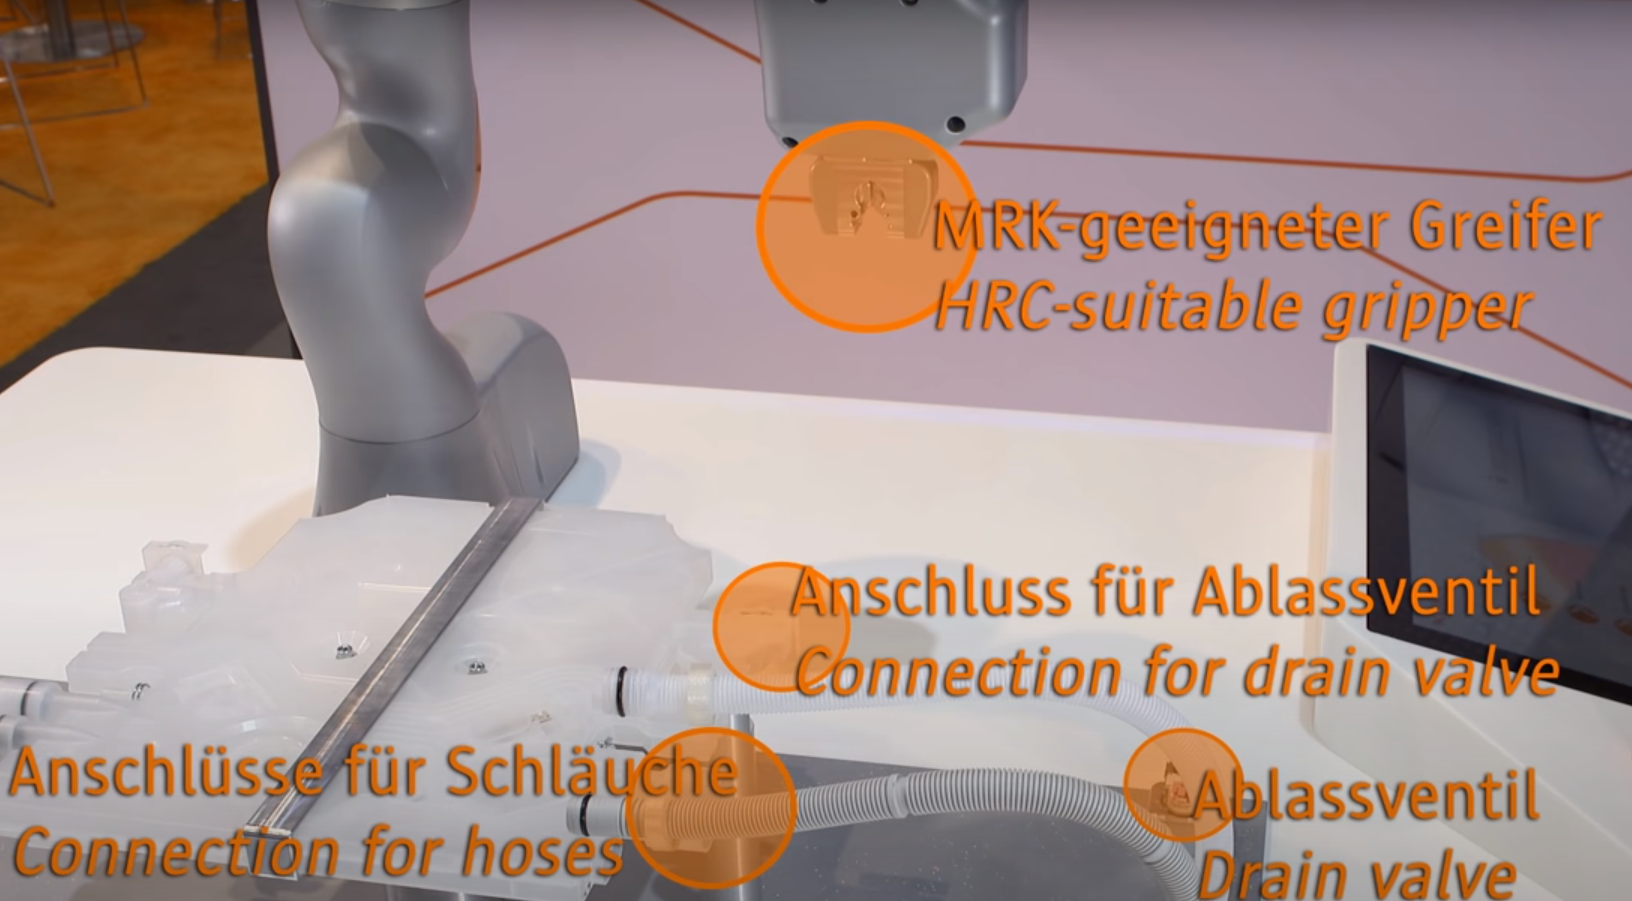
\includegraphics[scale=0.15]{kuka-setup-desc.png}
\caption{KUKA LBR iiwa in its workspace from the video}
\label{kuka-setup-desc}
\end{figure}

In the video, the robot is first shown in its workspace, showing a HRC-suitable
gripper. A drain valve, a connector for the drain valve, and a connection for
the hoses are shown. A still from the video describing the gripper and workspace is shown in Figure~\ref{kuka-setup-desc}.

After the setup is shown, the robot is shown performing the assembly tasks. The first
part shows the utilization of the joint torque sensors for process recognition. The second
part of the video shows the usage of the joint torque sensors for force-controlled
joining processes. The third part of the video shows the safety features of the robot.

Our objective in this paper is to analyze the robot kinematics and dynamics being
used in each of the three parts of the video. We will also describe how one would
simulate the tasks being performed by the robot in MATLAB, using the Robotics
ToolBox.

\section{Modeling and Analysis}

\subsection{MATLAB setup for robot}

We first describe the MATLAB setup for the robot. We use the Robotics Toolbox for
building the robot model. The robot model is built using the \texttt{rigidBodyTree} MATLAB type.
We use the KUKA LBR iiwa data sheet to populate the bodies and joints of the
\texttt{rigidBodyTree}. The bodies and joints are created using the \texttt{rigidBody} and
\texttt{rigidBodyJoint} functions in the Robotics Toolbox. At this point, we use
the DH parameters to assign fixed transforms to the joints, using the function
\texttt{setFixedTransform}.
The joints are attached to the bodies
using in the following way: \texttt{body1.Joint = joint1}. The bodies are then
attached to the tree structure by using the \texttt{addBody} function. The tree
can then be displayed using the \texttt{showdetails} function.
\subsection{Analysis of first part of video}

In this part of the video, the robot is shown performing a task where it correctly
finds the gripping point of the drain hose. The robot then picks up the drain hose,
traces the outline of the drain hose to the attached stopping point, and then inserts
the drain hose into the connection for the drain hose. It then repeats the same process
for a second drain hose.

\begin{figure}[h!]
    \centering
    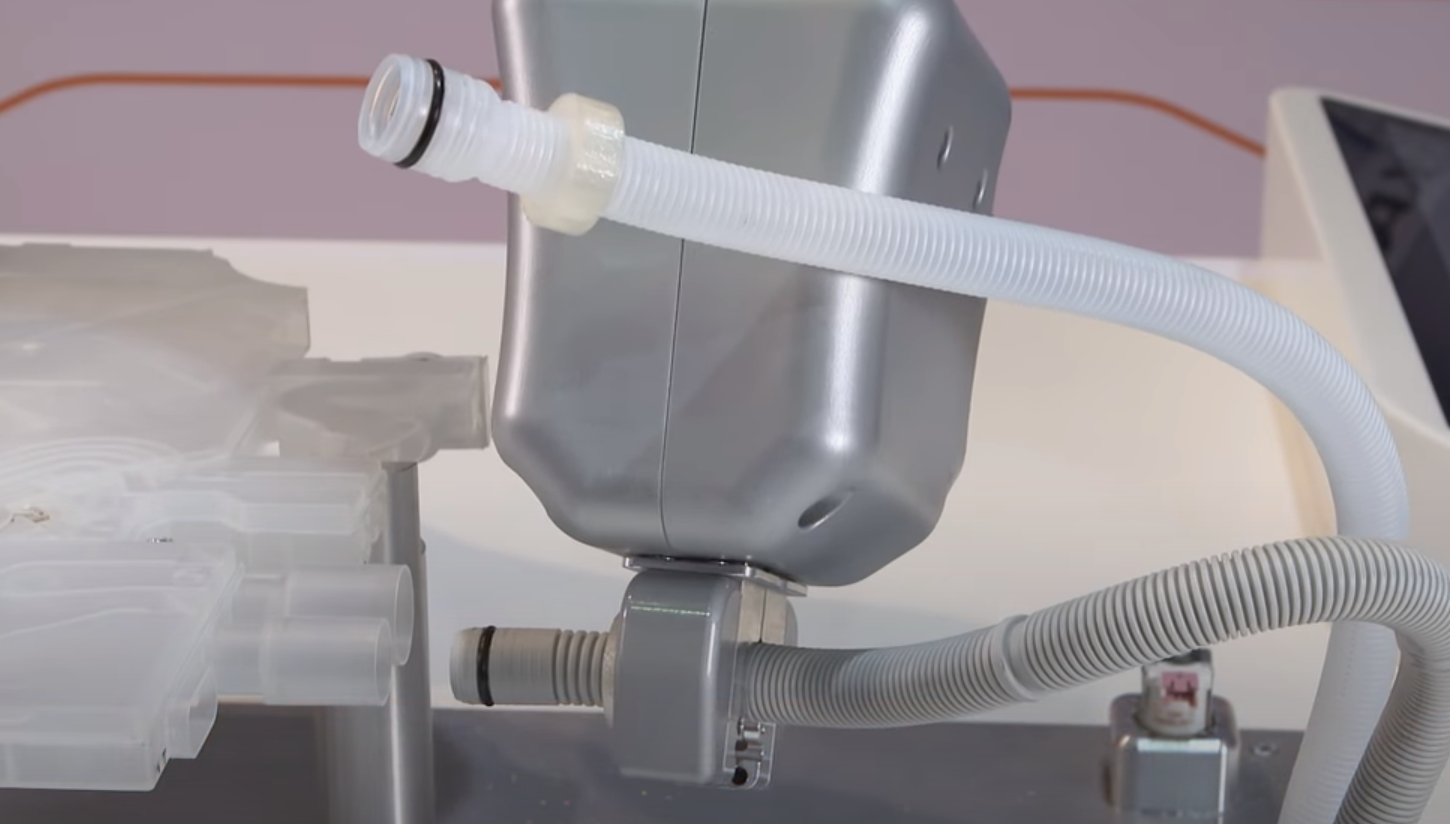
\includegraphics[scale=0.15]{kuka-drain-hose-insertion.png}
    \caption{Robot aiming to insert the first drain hose --- still from the video}
    \label{kuka-drain-hose-insertion}
\end{figure}

There are two key moments in this part of the video. The first is when the robot
uses its torque sensing to arrive at the `stopping point' in tracing the drain
hose, which helps it recognize the correct gripping point. The second is when
the robot is able to recognize the correct insertion point for the drain hose
using its torque sensing.

\subsubsection{Kinematics for first part of video}

The two main areas of kinematics that are used in this part of the video are
where the robot picks up the hoses, and where the robot inserts the hoses.
Specifically, we have a rough idea of where the hoses originate, so we would
use MATLAB's inverse kinematics solver to find the joint angles for the robot
required to pick up the hoses. For example, if the robot is named \texttt{robot} 
in our code, we declare our solver as \texttt{ik = inverseKinematics('RigidBodyTree',robot)}.
We then declare a $1 \times 7$ vector of pose tolerances, and an initial guess (which
would be our home position), and input it into the solver as \texttt{ik('body7',tform,weights,initialguess)},
where \texttt{tform} is the transform between the base frame and end-effector of our
robot, which is computed using \texttt{getTransform}. We would then use
\texttt{show(robot,configSoln)} to show the pickup position. If this looks correct,
then it would be our first goal position. We would then repeat this process for the
location where the robot inserts the hoses, which would become our second goal position.

\subsubsection{Dynamics for first part of video}

Once we have computed the goal joint positions using inverse kinematics, we begin 
to model our dynamics for the robot by implementing a force controller. We would
first set our goal position, and initialize our positions, velocities, and accelerations
to zero. We would then compute the joint torques using the \texttt{inverseDynamics}
function provided my MATLAB. For one of the arguments of this function, the current linear acceleration needs to be
computed, which can be obtained from the force needed for each joint. The force required
for each joint is modeled at the heart of our controller, given by the formula,

\[
    F = K_p E + K_d \dot{E}
\]

Where $E$ is the error computed from the difference between the current position and
the goal position. $K_p$ and $K_d$ are the proportional and derivative gains, respectively.
We can then compute the current velocities and positions by integrating the accelerations.
We can keep track of the joint torques and keep iterating our controller until we reach the first goal
position.

After the first goal position is reached, we similarly implement a velocity controller
which will move in a straight line in an `upward sloping direction' in order to find the
`stopping point' of the drain valve. The stopping point is found by using the live torque from
the joint torque sensors (an external wrench force will be detected). Then, we may go back to
our force controller to iterate towards the second goal position. The robot will detect that
the insertion is complete when another external counter-acting torque is detected on the end-effector.

\subsection{Analysis of second part of video}

In this part of the video, the robot is shown performing a task where it correctly
turns a drain valve to pick it up, and then inserts it into the connection for the
drain valve by also applying force to the drain valve and turning it. A still from
this part of the video is shown in Figure~\ref{kuka-drain-valve-insertion}.

\begin{figure}[h!]
    \centering
    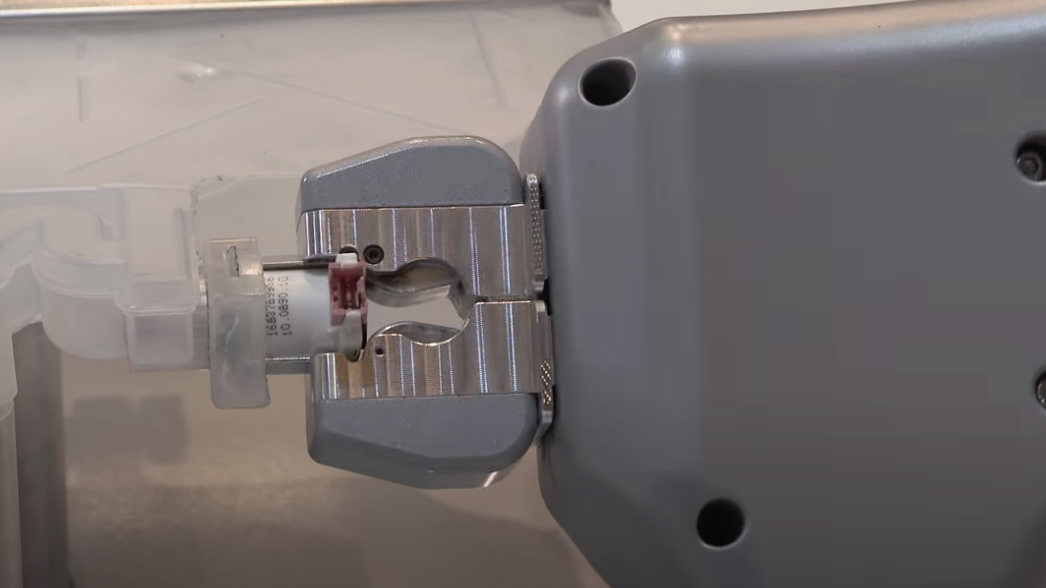
\includegraphics[scale=0.2]{kuka-valve-insertion.png}
    \caption{Robot turning the drain valve before insertion --- still from the video}
    \label{kuka-drain-valve-insertion}
\end{figure}

\subsubsection{Kinematics for second part of video}

The MATLAB functions and method, i.e., \texttt{inverseDynamics} and \texttt{getTransform} are used to compute the inverse kinematics for this part of the video is similar to the first part of the
video, except that we have new goal positions, and a new number of goal positions. We would
use inverse kinematics to first find the pickup location for the drain valve, which would be our
first goal. The second goal would be the `turned' position of the drain valve, which would be
our second goal. One thing to note during this turning is that a force is applied to the drain
valve, however this is not modeled in our kinematics --- it is modeled in our dynamics.
The third and fourth goals are similar in nature --- we need to find the target robot configuration for the the initial insertion location
for the drain valve, and the same for the final insertion location for the drain valve.

\subsubsection{Dynamics for second part of video}
For the dynamics, we will again use the force controller we described in the dyhamics for the first part
of the video. We will use the same formula for the force controller, however during the turning phases, we will need to use
our `inverseDynamics' function with the additional argument of the external wrench force. This external
wrench force is the force applied to the drain valve, which is modeled as a force applied to the end-effector
using the \texttt{externalForce} function. The external force is applied such that as though something
is `pulling away' the end-effector from the valve. This way, the end effector is able apply a force `into'
the valve, therefore aiding its turning.

During the non-turning phases, we will use the same force controller to arrive at goal
positions without any external wrench force.

\subsection{Analysis of third part of video}
In the third part of the video, it is demonstrated that the robot is able to perform its tasks
while observing human safety. It does this by maintaining a slow velocity, and by stopping
when it detects a human in its path. A still from this part of the video is shown in Figure~\ref{kuka-human-safety}.

To achieve these safety measures, we would need to adjust the gain values for our force controller
such that the robot moves slowly, i.e. approaches its goal position no faster than a certain period
of time.

\begin{figure}[h!]
    \centering
    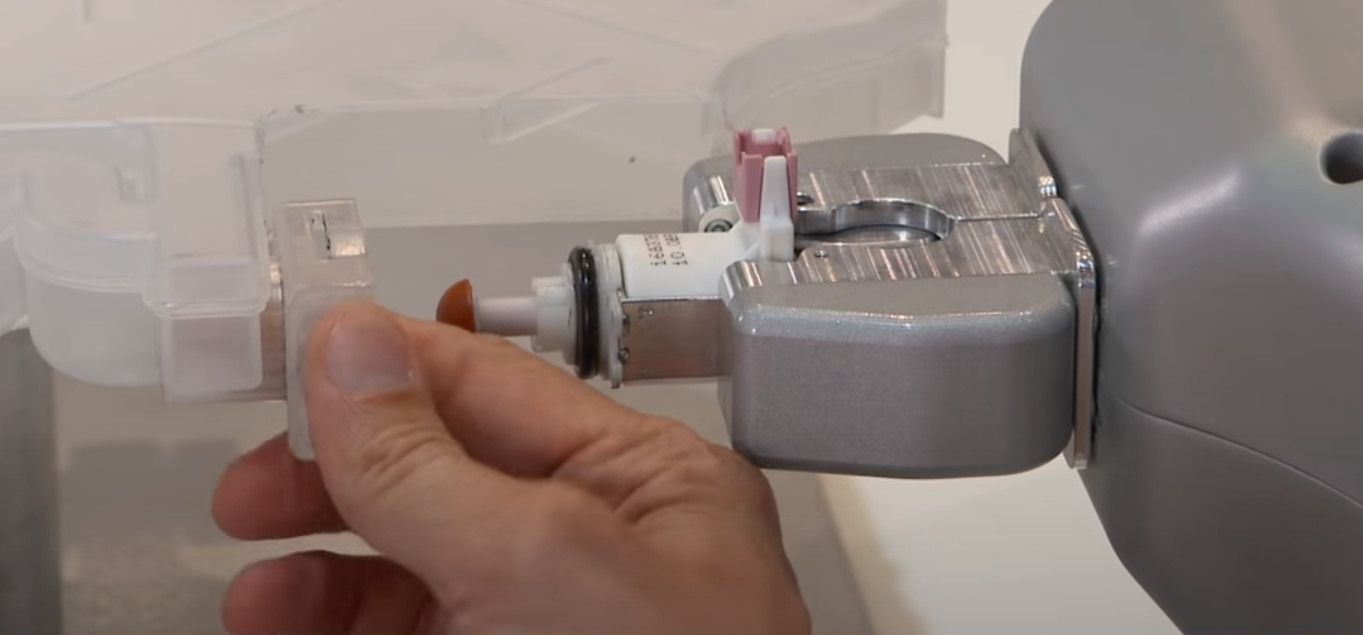
\includegraphics[scale=0.15]{kuka-human-safety.png}
    \caption{Robot stopping when it detects a human in its path --- still from the video}
    \label{kuka-human-safety}
\end{figure}
Furthermore, we would need to set up a test for this in MATLAB by using MATLAB's \texttt{addCollision} and
\texttt{checkCollision} functions. We would need to add a collision object to the robot, and then
check if the robot is colliding with the object. At the time of the collision, the velocity and resultant
force can be measured and compared to the safety standards. If the velocity and force are not within the
safety standards, we will need to continue to tune our force controller until it is within the safety standards.

\section{Conclusion}

In this paper, we have described the kinematics and dynamics of a KUKA LBR iiwa robot
that would be required to perform the tasks shown in the video. We have also described
how we would implement these kinematics and dynamics in MATLAB, and how we would test
collision safety in MATLAB.

\bibliography{refs.bib}
\bibliographystyle{IEEEtran}

\end{document}
